\documentclass[12pt]{article}
\usepackage[utf8]{inputenc}

\usepackage{lmodern}

\usepackage{enumitem}
\usepackage[margin=2cm]{geometry}

\usepackage{amsmath, amsfonts, amssymb}
\usepackage{graphicx}
%\usepackage{subfigure}
\usepackage{tikz}
\usepackage{pgfplots}
\usepackage{multicol}

\usepackage{comment}
\usepackage{url}
\usepackage{calc}
\usepackage{subcaption}
\usepackage[indent=0pt]{parskip}
\usepackage{animate}

\usepackage{array}
\usepackage{blkarray,booktabs, bigstrut}
\usepackage{bigints}

\pgfplotsset{compat=1.16}

% MATH commands
\newcommand{\ga}{\left\langle}
\newcommand{\da}{\right\rangle}
\newcommand{\oa}{\left\lbrace}
\newcommand{\fa}{\right\rbrace}
\newcommand{\oc}{\left[}
\newcommand{\fc}{\right]}
\newcommand{\op}{\left(}
\newcommand{\fp}{\right)}

\newcommand{\bi}{\mathbf{i}}
\newcommand{\bj}{\mathbf{j}}
\newcommand{\bk}{\mathbf{k}}
\newcommand{\bF}{\mathbf{F}}

\newcommand{\mR}{\mathbb{R}}

\newcommand{\ra}{\rightarrow}
\newcommand{\Ra}{\Rightarrow}

\newcommand{\sech}{\mathrm{sech}\,}
\newcommand{\csch}{\mathrm{csch}\,}
\newcommand{\curl}{\mathrm{curl}\,}
\newcommand{\dive}{\mathrm{div}\,}

\newcommand{\ve}{\varepsilon}
\newcommand{\spc}{\vspace*{0.5cm}}

\DeclareMathOperator{\Ran}{Ran}
\DeclareMathOperator{\Dom}{Dom}

\newcommand{\exo}[1]{\noindent\textcolor{red}{\fbox{\textbf{Problem {#1}}}\hrulefill}\\\\ }
\newcommand{\qu}[4]{\noindent\textcolor{#4}{\fbox{\textbf{Section {#1} | Problem {#2}}} \hrulefill{{\fbox{\textbf{{#3} Points}}}}\\}}

\newcommand{\semester}{Fall 2023}

\newcommand{\CVup}{%
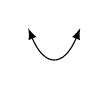
\begin{tikzpicture}
\draw[black, <->, >=latex] (-0.33, 0.5) .. controls (-0.125, 0) and (0.125, 0) .. (0.33, 0.5);
\end{tikzpicture}}

\newcommand{\CVupInc}{%
\begin{tikzpicture}
\draw[black, ->, >=latex] (0,0) .. controls (0.2, 0) and (0.4, 0.2) .. (0.5, 0.5);
\end{tikzpicture}}

\newcommand{\CVupDec}{%
\begin{tikzpicture}[rotate=270]
\draw[black, ->, >=latex] (0,0) .. controls (0.2, 0) and (0.4, 0.2) .. (0.5, 0.5);
\end{tikzpicture}}

\newcommand{\CVdown}{%
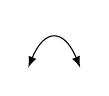
\begin{tikzpicture}
\draw[black, <->, >=latex] (-0.33, -0.5) .. controls (-0.125, 0) and (0.125, 0) .. (0.33, -0.5);
\end{tikzpicture}}

\newcommand{\CVdownInc}{%
\begin{tikzpicture}
\draw[black, ->, >=latex] (-0.5, -0.5) .. controls (-0.5, -0.3) and (-0.5, -0.1) .. (0,0);
\end{tikzpicture}}

\newcommand{\CVdownDec}{%
\begin{tikzpicture}[rotate=-90]
\draw[black, ->, >=latex] (-0.5, -0.5) .. controls (-0.5, -0.3) and (-0.5, -0.1) .. (0,0);
\end{tikzpicture}}

\begin{document}
	\noindent \hrulefill \\
	MATH-244 \semester \hfill Practice Problems Solutions\\
	Section 15.4 \hfill Pierre-Olivier Paris{\'e} \\\vspace*{-1cm}
	
	\noindent\hrulefill
	
	\spc	

	\exo{8}
	\\
	The shape of the lamina is shown in the picture below.
		\begin{figure}[h]
		\centering
		\includegraphics[scale=0.5]{exo8_15-4.png}
		\end{figure}
	So we get
		\begin{align*}
		D = \{ (x, y) \, : \, -1 \leq x \leq 2 \text{ and } x^2 \leq y \leq x + 2 \}. 
		\end{align*}
	
	The density is $\phi (x) = k x^2$ for some constant $k$. Then
		\begin{align*}
		M = \int_{-1}^2 \int_{x^2}^{x + 2} k x^2 \, dy dx = 63k/20.
		\end{align*}
		
	The center of mass is given by $(\overline{x} , \overline{y})$. We then compute
		\begin{align*}
		\overline{x} = \frac{20}{63k} \int_{-1}^2 \int_{x^2}^{x + 2} k x^3 \, dy dx = \frac{20}{63} \times \frac{18}{5} = \frac{8}{7} .
		\end{align*}
	and
		\begin{align*}
		\overline{y} = \frac{20}{63} \int_{-1}^2 \int_{x^2}^{x + 2} x^2 y \, dy dx =  \frac{20}{63} \times \frac{531}{70} = \frac{118}{49} .
		\end{align*}
	So the center of mass is $(\overline{x}, \overline{y}) = (8/7 , 118/49 )$. 

	\spc
	
	\exo{12 (only the mass)}
	\\
	We have $\rho (x, y) = k (x^2 + y^2 )$. In polar coordinate, the disk is described as followed
		\begin{align*}
		D = \{ (r, \theta ) \, : \, 0 \leq r \leq 1 \text{ and } 0 \leq \theta \leq \pi/2 \} .
		\end{align*}
	Setting $x = r\cos \theta$ and $y = r \sin \theta$, we have $dA = r dr d\theta$ and so
		\begin{align*}
		M = \iint_D \rho (x, y ) \, dA = \int_0^{\pi/2} \int_0^1 k r^2 r \, dr d\theta = k \pi / 8 .
		\end{align*}
	
	\spc
	
	\exo{20}
	\\
	The fan is a suare with sides of length $2$ with the lower left corner positioned at the origin, so
		\begin{align*}
		D = [0, 2] \times [0, 2] .
		\end{align*}
	We have to compare $I_x$ and $I_y$.
	
	Firstly, we have
		\begin{align*}
		I_x = \iint_D y^2 \rho (x, y) \, dA = \int_0^2 \int_0^2 y^2 (1 + 0.1 x) \, dx dy = 88/15 .
		\end{align*}
	Secondly, we have
		\begin{align*}
		I_y = \iint_D x^2 \rho (x, y) \, dA = \int_0^2 \int_0^2 x^2 (1 + 0.1 x) \, dx dy = 92/15 .
		\end{align*}
	We see that $I_y > I_x$, and so it would be more difficult to rotate the fan blade around the $y$-axis.


\end{document}